%       $Id: tabellen.tex,v 1.13 2004/05/23 10:56:44 bronger Exp $    
%
%     tabellen.tex -- Part of the LaTeX Tutorium
%     Copyright 2004 Project Members of
%                    https://github.com/latextemplates/latex-tutorium/
%                    
%
%   This program is free software; you can redistribute it and/or
%   modify it under the terms of the Artistic License 2.0 as published
%   by Larry Wall.  You should have received a copy of the Artistic
%   License 2.0 along with this program in the file COPYING; if not,
%   you can get it at
%     http://dev.perl.org/rfc/346.html
%   or contact the current maintainers of the LaTeX Tutorium.
%
%   This program is distributed in the hope that it will be useful, but
%   WITHOUT ANY WARRANTY; without even the implied warranty of
%   MERCHANTABILITY or FITNESS FOR A PARTICULAR PURPOSE.  See the
%   Artistic License 2.0 for more details.
%
%   This file may only be distributed together with a copy of the LaTeX
%   Turorium.
%
%   The LaTeX Tutorium consists of all files listed in manifest.txt.

\section{Tabellen}

Um eine Tabelle einzuf�gen, sind drei Schritte notwendig.
\begin{enumerate}
\item Im Men� "`Einf�gen--Tabelle"' w�hlen.  Entscheiden, ob die Tabelle
  "`gleiten"' soll oder nicht (s.\,u.).  Als Ergebnis wird eine leere
  Rumpf-Tabelle in das Dokument eingef�gt.
\item Die Zahl der Spalten und die Spalten-Ausrichtung angeben.
\item Die Zeilen und Spalten der Tabelle eingeben.
\end{enumerate}

Betrachten wir die folgende Beispiel-Tabelle:
\begin{center}
  \begin{tabular}{llc}
    \toprule
    Sternname   &  Sternbild  &  Entfernung (Lj) \\
    \midrule
    Rigel       &  Orion      &     780          \\
    Acturus     &  Bo�tes     &      37          \\
    Deneb       &  Schwan     &    3200          \\
    Rigil Kent  &  Zentaur    &      4,4         \\
    \bottomrule             
  \end{tabular}
\end{center}

\begin{figure}
  \centering
  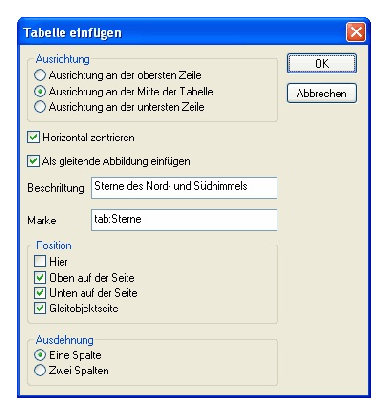
\includegraphics{tabelle2}
  \caption{Einf�gen einer gleitenden Tabelle}
  \label{fig:Gleittabelle}
\end{figure}

Um das einzugeben, w�hlt man im Men� "`Einf�gen--Tabelle"' oder dr�ckt
\Alt+\Ctrl+\mbox{\keystroke T\@.}  Es �ffnet sich das Dialog-Fenster in
Abbildung~\ref{fig:Gleittabelle}.  Dort kann man noch eine Beschriftung und
eine Marke eingeben (f�r Querverweise, siehe Seite~\pageref{sec:Querverweise}),
und muss auf "`OK"' dr�cken.  Der Editor f�gt dann automatisch eine Art Rumpf
f�r die Tabelle ein:
\begin{lstlisting}[escapeinside=`']
\begin{table}
  \centering
  \begin{tabular}
    `\textrm{\emph{(Hier stehen die Zeilen und Spalten)}}'
  \end{tabular}
  \caption{Sterne des Nord- und S�dhimmels}
  \label{tab:Sterne}
\end{table}
\end{lstlisting}
Als n�chstes m�ssen wir \LaTeX{} sagen, wieviele Spalten unsere Tabelle haben
soll.  In unserem Fall sind es offensichtlich drei.  Also schreibe ich ein
"`\lstinline|{llc}|"' hinter das \lstinline|\begin{tabular}|:
\begin{lstlisting}
  ...
  \begin{tabular}{llc}
    ...
\end{lstlisting}
Jeder der drei Buchstaben steht f�r eine Spalte.  Ein "`l"' bedeutet
\emph{linksb�ndige} Ausrichtung.  Entsprechend stehen "`r"' und "`c"' fuer
\emph{rechtsb�ndig} und \emph{zentriert}.  F�r unser Beispiel sollen also die
ersten beiden Spalten links ausgerichtet werden, und die letzte zentriert.

Jetzt kann man die Tabelle mit Inhalt f�llen.  Tabellen werden zeilenweise
eingegeben.  Spalten trennt man mit "`\&"'"~Zei\-chen, Zeilen m�ssen mit
"`\verb|\\|"' beendet werden:
\begin{lstlisting}[basicstyle=\ttfamily\ifminion\else\footnotesize\fi]
  ...
  \begin{tabular}{llc}
    \toprule
    Sternname   &  Sternbild  &  Entfernung (Lj) \\
    \midrule
    Rigel       &  Orion      &     780          \\
    Acturus     &  Bo�tes     &      37          \\
    Deneb       &  Schwan     &    3200          \\
    Rigil Kent  &  Zentaur    &      4,4         \\
    \bottomrule             
  \end{tabular}
  ...
\end{lstlisting}
\lstinline{\toprule}, \lstinline{\midrule} und \lstinline{\bottomrule} erzeugen
die obere, mittlere und untere Linie in der Tabelle.

\begin{table}
  \centering
  \begin{tabular}{llc}
    \toprule
    Sternname   &  Sternbild  &  Entfernung (Lj) \\
    \midrule
    Rigel       &  Orion      &     780          \\
    Acturus     &  Bo�tes     &      37          \\
    Deneb       &  Schwan     &    3200          \\
    Rigil Kent  &  Zentaur    &      4,4         \\
    \bottomrule             
  \end{tabular}
  \caption{Sterne des Nord- und S�dhimmels}
  \label{tab:Sterne}
\end{table}

\nopagebreak
Das Ergebnis sieht man in Tabelle~\vref{tab:Sterne}.  Tabellen sind in \LaTeX{}
am Anfang etwas einsch�chternd, aber man gew�hnt sich recht schnell daran.


\subsection{Gleitende und nicht-gleitende Tabellen}
\label{sec:Gleittabellen}

Genauso wie auch bei Abbildungen gibt es \emph{gleitende} und
\emph{nicht-gleitende} Tabellen.  Wir haben oben eine gleitende Tabelle
eingef�gt, d.\,h.\ sie kann eine Beschriftung haben, und \LaTeX{} sucht
selbstst�ndig den besten Platz f�r sie.  Das ganze ist v�llig analog zu
Abbildungen, siehe Abschnitt~\vref{sec:Gleitobjekte}.


%%% Local Variables: 
%%% mode: latex
%%% TeX-master: "latex-tutorium"
%%% End: 
